\documentclass[conference]{IEEEtran}

\IEEEoverridecommandlockouts

\usepackage{setspace}
\usepackage{enumerate}
\usepackage{cite}
\usepackage{times}
\usepackage{url}
\usepackage{graphicx}
\usepackage{subfigure}
\usepackage{amsmath}
\usepackage[ruled,vlined,linesnumbered]{algorithm2e}
\usepackage{listings}
\setlength{\belowdisplayskip}{0pt} \setlength{\belowdisplayshortskip}{0pt}
\setlength{\abovedisplayskip}{0pt} \setlength{\abovedisplayshortskip}{0pt}
\usepackage{makecell}

\lstset{language=C}
\newcommand\foo{\lstinline{t}}\newcommand\foobar[2][]{\lstinline[#1]{#2}}

\graphicspath{ {img/} }


\begin{document}
\title{Parallel Enhanced Whale Optimization Algorithm}

\author{
\IEEEauthorblockN{
Bevan Stanely
}
\IEEEauthorblockA{Department of Microbiology and Cell Biology\\
Indian Institute of Science, Bangalore, India\\
bevanstanely@iisc.ac.in}
}

\maketitle

\begin{abstract}

    One of the current state-of-the-art nature-inspired meta-heuristic optimization algorithms is the enhanced Whale Optimization Algorithm (WOAmM). 
    It integrates a modified mutualism phase from Symbiotic Organisms Search (SOS) into the original Whale Optimization Algorithm (WOA). 
    As a result, it efficiently addresses the premature convergence seen in WOA. 
    We propose a parallel implementation of the same under the CUDA GPU architecture and demonstrate the speedups achieved compared to the sequential algorithm.

\end{abstract}

\section{Introduction}
\label{intro}

Meta-heuristic algorithms work by spawning a population of agents and engaging them in exploration and exploitation phases. 
The exploratory phase helps to explore the search space extensively, whereas the exploitatory step refines promising solutions from the exploratory stage. 
Two primary challenges for parallel meta-heuristic algorithms are generating thread-safe random numbers and resolving data dependencies among populations. 
Additionally, we fixed the population size to that of warp size and resorted to using only the registers’ local memory for improved cache efficiency, 
allowing us to employ the fast warp primitives for intra-warp communication and evade the slow shared memory altogether.

\section{Related Work}

Meta-heuristic algorithms are iterative by nature, and swarm-based methods, in particular, 
preserve search space information over subsequent iterations and involve fewer operators compared to evolutionary approaches. 
Mirjalili and Lewis \cite{MIRJALILI201651} described a swarm-based meta-heuristic optimization algorithm called Whale Optimization Algorithm (WOA). 
It is inspired by the bubble-net hunting strategy of humpback whales. 
A hybrid of WOA with a modified mutualism phase from Symbiotic Organisms Search (SOS) came out designated enhanced Whale Optimization Algorithm (WOAmM)\cite{CHAKRABORTY2021107086}. 
WOAmM addresses the drawbacks of WOA, namely, low exploration ability, slow convergence speed, and being trapped into a local solution easily.

\section{A Parallel Enhanced Whale Optimization Algorithm}

WOAmM has two components: 
the original WOA and the Mutualism phase of the symbiotic organism search (mSOS) algorithm. 
Sequential execution of WOAmM allowed data-dependent stochasticity for both components. 
The probability that a randomly selected individual has already been updated increases from zero for the first individual to one for the last individual in serial WOAmM. 
A parallel implementation of the algorithm will have to forsake this advantage. 
But as would be later found, this is inconsequential for the optimization if we can assure the quality of random numbers.

\subsection{Mutualism phase of the symbiotic organism search (mSOS) algorithm}

Mutualism is a two-way relationship between two organisms, where both of them benefitted from the interaction. 
A typical example would be honey bees and flowers. 
Mathematically we can express it as,

\setlength{\arraycolsep}{0.0em}
\begin{eqnarray}
    P^{(k+1)}_i= P^{(k)}_i+rnd\cdot(P_s - MV\cdot BF1)\\
    P^{(k+1)}_r= P^{(k)}_n+rnd\cdot(P_s - MV\cdot BF2)
\end{eqnarray}
\setlength{\arraycolsep}{0pt}

where $P_i$ is the $i^{th}$ individual\footnote{$P_*$ corresponds to a position vector}, and $P_r$ is an organism randomly\footnote{We use $rnd$ to denote a random number with a uniform distribution between $[0, 1]$. All references to random numbers in this paper corresponds to $rnd$} selected to interact with $P_i$ and $P_s$ is the individual with the best fitness among $P_r \And P_s$. 
The remaining variables are as follows.

\setlength{\arraycolsep}{0em}
\begin{eqnarray}
    P_s=min fitness(P_n,P_m) \\
    P_r=max fitness(P_n,P_m) \\
    MV = \frac{P_i+P_s}{2} \\
    BF = round(1+rnd)
\end{eqnarray}
\setlength{\arraycolsep}{0pt}

\subsection{Whale Optimization Algorithm (WOA)}

WOA mimics the bubble-net hunting strategy of humpback whales and includes three phases, searching the prey, encircling the target, and spiral bubble-net feeding maneuver. 
WOA uses these three phases to balance be­tween exploration and exploitation.

\subsubsection{Searching the prey}

Whales randomly search the target, depending on its current location. 
This behavior of the humpback whale is used in the algorithm to amplify its exploration capability.

\subsubsection{Encircling the prey}

During this phase, we assume the current best solution to be close to the optimal solution. 
Then, the whales update their positions near the best solutions.

We can mathematically write 1 and 2 as:

\setlength{\arraycolsep}{0em}
\begin{eqnarray}
    P^{(k+1)}=P^{(k)}_{random/best}-A\cdot \overline{D}
\end{eqnarray}
\setlength{\arraycolsep}{0pt}

The vectors $A$, $C$, and $\overline{D}$ are calculated as follows:

\setlength{\arraycolsep}{0em}
\begin{eqnarray}
    \overline{D}=| C\cdot P^{(k)}_{random/best}-P^{(k)}| \\
    A = 2a_1 \times rnd - a_1 \\
    C = 2 \times rnd
\end{eqnarray}
\setlength{\arraycolsep}{0pt}

\begin{figure}[ht]
    \centering
    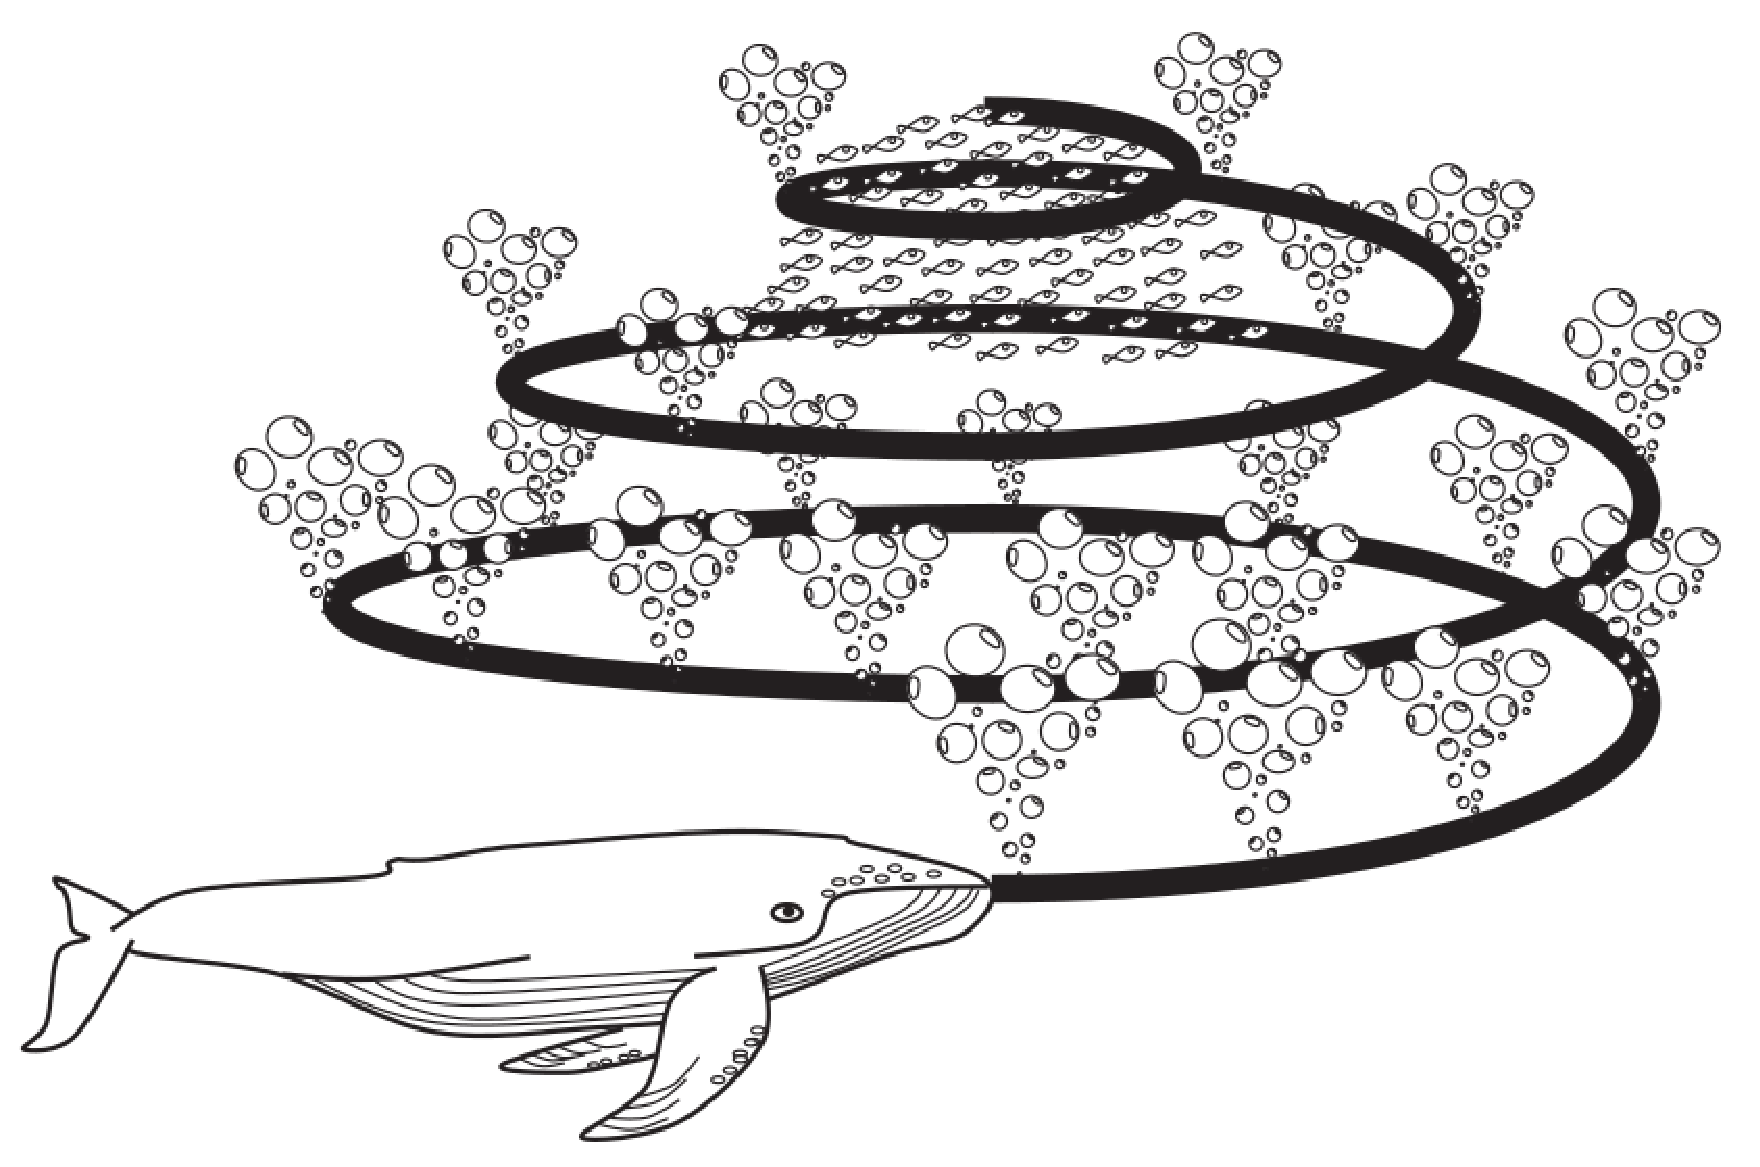
\includegraphics[width=0.4\textwidth]{bubble-net}
    \caption{Bubble-net feeding behavior of humpback whales.}
    \label{fig:bubble-net}
\end{figure}

\subsubsection{Bubble-net attacking strategy}

Humpback whales follow a surface feeding behavior known as bubble-net attack, where the whales move on a helix-shaped path. 
We implement this strategy in WOA as:

\setlength{\arraycolsep}{0em}
\begin{eqnarray}
    P^{(k+1)}= D^*\cdot e^{bl} \cdot \cos{2\pi l} + P^{(k)}_{best}\\
    D^*= P^{(k)}_{best}-P^{(k)}
\end{eqnarray}
\setlength{\arraycolsep}{0pt}

\begin{table}[!t]
    \renewcommand{\arraystretch}{1.3}
    \caption{Parameters of WOA}
    \label{table_example}
    \centering
    \begin{tabular}{c}
    \(a_1\): A number decreasing linearly from 2 to 0\\
    \(a_2\): A number decreasing linearly from -1 to -2 \\
    \(b=1\) \\
    \(l = (a_2 - 1)rnd + 1\) \\
        \hline
    \end{tabular}
\end{table}

\begin{algorithm}
    \SetAlgoLined
        \# Start kernel from here for single warp\;
        \For{each thread}{
        Initialize the population $P_i(i = 1,2\ldots n)$\;
        Initialize $k = 0 \And \max_{iter}$\;
        \While{$k < \max_{iter}$}{
            Fetch population = $[P_m , P_n]$ from other threads randomly, where $P_i \neq P_s \neq P_r$\;
            Calculate the new value of $P_i \And P_r$ using eq.1 and eq.2\;
            Calculate the fitness of $P_i^{k+1}$ and $P_r^{k+1}$\;
            Update the value of $P_i$ and $P_r$if the new fitness value is minimum\;
        
            Find $P_{best}$\;
        \#Procedure WOA starts from here\;
        \For{every \textit{search-agent}}{
            Update $A,C,l \And \beta$\;
            \eIf{$\beta < 0.5$}{
                Array = $[P_{rnd},P_{best}]$
                Index int ind = $|A| \geq 1$
                Update the position of current \textit{search-agent} by eq.2 or 6
            }{
                Update the position of current \textit{search-agent} by eq.8
            }
            Check boundary conditions\;
        }
        $k=k+1$
        }
        }
        Return $P_{best}$
        \caption{Parallel WOAmM for GPU.}
    \end{algorithm}

\subsection{Parallelization}

For parallelization, we employed CUDA under GPU. 
We modeled the individuals $P_i$ of the population as GPU threads and stored the population data and its fitness in the thread’s local memory (register). 
To capitalize on the wrap level communication offered, we fixed the population size $n$ to the warp size 32, allowing communication of population data without involving the slow shared memory. 
A single kernel executed the complete WOAmM algorithm within a thread warp.

\subsubsection{Intra-warp Communication}

Threads need to communicate to find $P_{best}$ and to find $P_{random}$. 
We have resorted to an all-to-all butterfly reduction with \lstinline{__shfl_xor_sync()} warp primitive to find $P_{best}$, which returns the cost and thread id of the best. 
Similarly, for $P_{random}$, we calculate the thread id first. 
Later for both cases, we use \lstinline{__shfl_sync()} warp primitive to fetch the individual $P_{best}$ or $P_{random}$.

\subsubsection{Avoiding Warp Divergence}

mSOS and WOA have conditionals that can lead to warp divergence. 
We have used pointer arrays and binary boolean values to prevent it.

\subsubsection{Random Numbers}

WOAmM is a stochastic algorithm and hence needs random numbers for execution. 
The state size of the Mersenne Twister 19937 generator (64 bit) that we use in a sequential program is 19937 bits or 2.5 kilobytes. 
In parallel execution for thread safety, we need a state for each thread. 
Hence the pseudo-random number generators like \lstinline{mt19937_64} from the CPU world are not ideal; the local memory for GPUs will become a bottleneck. 
Therefore we have used two RNGs \lstinline{MRG32k3a}, and \lstinline{Philox_4x32_10}, with device API, which is much leaner and a  robust RNG from the Mersenne Twister family \lstinline{MTGP32} with host API.
We initialized the device RNGs within the CUDA kernel and used the sequence option to distribute states for individual threads.  
We initialized the host RNG from the CPU.

\begin{table*}[!t]\renewcommand{\arraystretch}{1.3}
    \caption{Fixed dimension unimodal and multimodal functions.}
    \label{tbl:func}
    \centering
    \begin{tabular}{c||c||c||c||c||c||c}
    \hline\bfseries ID & \bfseries Function & \bfseries Equation & \bfseries Search Space & \bfseries Dimension D & \bfseries Optimum Value\\
    \hline \multicolumn{6}{c}{Unimodal} \\
    \hline F1 & Sphere & \(F(x)=\sum_{k=1}^Dx_k^2\) & \([-100,100]\)&30&0\\
    \hline
    \hline F2 & Rosenbrock & \(F(x)=\sum_{k=1}^{D-1}[100(x_{k-1}-x_k^2)^2+(x_k-1)^2\) & \([-30,30]\)&30&0\\
    \hline
    \hline \multicolumn{6}{c}{Multimodal} \\
    \hline F3 & Rastrigin & \(F(x)=\sum_{k=1}^{D}[x_k^2-10\cos(2\Pi x)+10]\) & \([-5.12,5.12]\)&30&0\\
    \hline
    \hline F4 & Griewank & \(F(x)=\frac{1}{4000}\sum_{k=1}^{D}x_k^2-\prod_{k=1}^D\cos(\frac{x_k}{\sqrt{k}})+1\) & \([-600,600]\)&30&0\\
    \hline
\end{tabular}
\end{table*}

\section{Experiments and Results}

\subsection{Experiment Setup}

Parallel WOAmM was evaluated by applying it to four well-known multi-variate functions selected from the original paper. 
The sample included two unimodal (F1 and F2) and two multimodal (F3 and F4) functions with dimensions 30. 
Further information regarding the functions is available in Table ~\ref{tbl:func}.

For an optimization algorithm, while parallelizing, we have to focus on the accuracy of the result and execution speed. 
Thus, we face two main challenges to achieve our goal. 
First, we have to make up for the loss of data dependency and then address the lower quality of GPU RNGs. 
Hence for the experiments, we have varied three parameters. 
They are as follows:

\begin{enumerate}
    \item Types of RNGs.
    \item Number of iterations of WOAmM
    \item Number of blocks that run simultaneously in a single experiment
\end{enumerate}

The exact details of the parameters are available in Table ~\ref{tbl:parameters}.

\begin{table}[!t]\renewcommand{\arraystretch}{1.3}
    \caption{Parameters Varied in the Experiments}
    \label{tbl:parameters}
    \centering
    \begin{tabular}{c||c}
    \hline\bfseries Parameter & \bfseries Set\\
    \hline
    \hline RNG & \makecell{Host: \foobar[language=C]{\{MTGP32\}} \\ Device: \foobar[language=C]{\{MRG32k3a,Philox_4x32_10\}}}\\
    \hline
    \hline \# Iterations & \foobar[language=C]{\{30,100,300\}} \\
    \hline
    \hline \# Blocks & \foobar[language=C]{\{1,2,4,6\}} \\
    \hline
\end{tabular}
\end{table}

We implemented Parallel WOAmM, compared optimization efficiency with the sequential algorithm, and then analyzed the speed-up to the sequential algorithm with 30 iterations of WOAmM across all parameters. 
All the experiments were performed with the GPU node of CDS Turing Cluster, with NVIDIA Tesla K40M GPU and Xeon E5 2620 V2 CPU with 24 GB memory.

To effectively compare device RNGs with host RNG for the Parallel WOAmM, we have separated RNG state initialization from the actual execution of Parallel WOAmM. 
Hence the memory allocation and RNG initialization times are not included in the total runtime of Parallel WOAmM. 
However, the total runtime includes computation costs with memory copy call from device to host.

The efficiency of Parallel WOAmM has been measured by comparing it to the sequential counterpart. For Parallel WOAmM, we collected data for executions with four functions by varying parameters. 
Thus, each execution of the algorithm for a particular function was carried out 50 times.

\begin{figure}[ht]
    \centering
    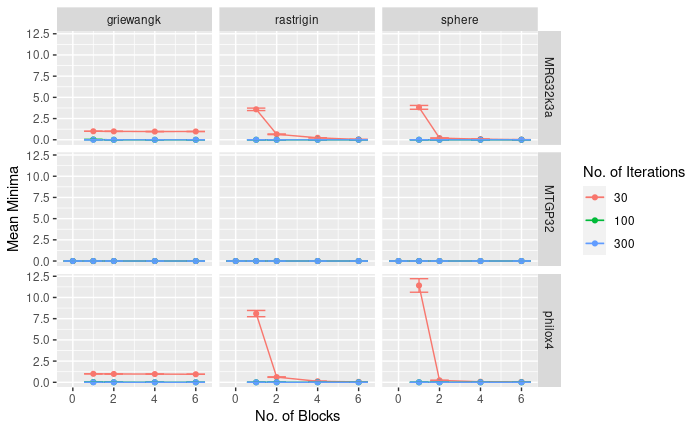
\includegraphics[width=0.44\textwidth]{fitness}
    \caption{The mean value of evaluated function with error bars. Optimal value is 0. Note sequential program(MT64 RNG) is included under MTGP32 for comparison as block 0.}
    \label{fig:fitness}
\end{figure}

\subsection{Results}

Figure ~\ref{fig:fitness} summarizes the optimization efficiency of the Parallel WOAmM compared against sequential execution for variable parameters. 
We have excluded F2 from the results as the optimization of single block Parallel WOAmM with \lstinline{Philox_4x32_10} was significantly less efficient and hid the variations in other experiments.

\begin{figure}[ht]
\centering
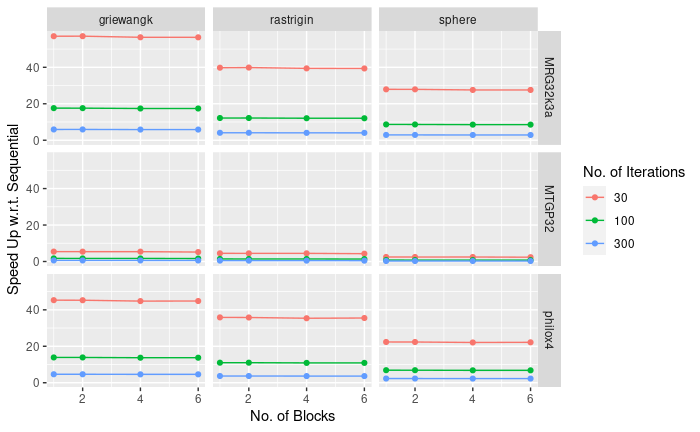
\includegraphics[width=0.44\textwidth]{speed_up}
\caption{Speed-ups of parallel implementations w.r.t. sequential program with 30 iterations and MT64 RNG}
\end{figure}

Have one para for conclusions and one para for future work.

\bibliographystyle{IEEEtran}
\bibliography{bevan_report}

\end{document}

